\section{Accuracy Analysis}
\label{sec:accuracy}

% 1. Write about using training data as best of the history here and in \S\ref{sec:study}.\\ 
% 2. Argument for using the 2Sigma trace as the main
% evaluation trace and other answers about the trace diversity here and in
% \S\ref{sec:study}.}

In this section, we perform an in-depth study of the prediction
accuracy of the two learning approaches: {\em learning in time}
(history-based learning) and {\em learning in space}
(task-sampling-based learning).  
{
Both approaches can potentially be used
to learn  different job properties for different optimization objectives.
In this paper, we focus on job completion time 
because it is an important metric that has been intensively studied
in recent work~\cite{cora:infocom2015,DontCryOverSpilledRecords,kairos:socc2018,varys:sigcomm14,corral,3Sigma,AltruisticScheduling,aalo:sigcomm15}.
}


We first derive analytical bounds on
their prediction errors (\S\ref{sec:accuracy:quantity}).  We then
measure and compare the bounds in real traces from two production
datacenters (\S\ref{sec:accuracy:trace}).  Finally, we
experimentally compare the prediction accuracy of learning in space
with a history-based predictor
\primarybasepredict~\cite{3Sigma} in estimating the job runtimes
(\S\ref{sec:accuracy:experiment}).
We pick \primarybasepredict because it is a state-of-the-art 
history-based predictor that can learn for non-recurrent jobs.

%  , and thus specific choices are somewhat orthogonal to the main focus of our
%  paper, which is to show that sampling-based prediction can be a viable
%  alternative to history-based prediction, explain the situations where
%  it will work well, and demonstrate its effectiveness empirically
%  through production traces. 
% Consistent with this objective, we mainly focus on estimating task running-times.

\subsection{Quantitative Comparison}
\label{sec:accuracy:quantity}

We first  present a theoretical analysis to compare the two
approaches. We caution that here we use a highly-stylized model (e.g., two
jobs and normal task-length distributions), which does not capture the
possible complexity in real clusters, such as heavy parallelism across servers and highly-skewed 
task-length distributions. Nonetheless, it reveals important insights
that help us understand in which regimes history-based schemes or sampling-based
schemes will perform better. Consider a simple case of two jobs
$j_1$ and $j_2$, where each job has $n$ tasks. The size of each task of $j_1$
is known. Without loss of generality, let us assume that the task size of $j_1$
is 1. Thus, the total size of $j_1$ is $n$. The size of a task of $j_2$ is
however unknown. Instead, we know the following about $j_2$: 
%  \editaj{(1) The average
%  task size across all tasks of $j_2$, denoted by $x$, follows a normal
%  distribution with mean $\mu$ and variance $\sigmanotsqrd$;}{
(1) The average
task size of $j_2$, denoted by $x$, follows a normal
distribution with mean $\mu$ and variance $\sigmanotsqrd$;
(2) Given $x$, the size of a random task of the job follows a normal 
distribution with mean $x$ and variance $\sigmaonesqrd$.
Intuitively, $\sigmanotsqrd$ captures the variation of mean
task-lengths \emph{across} many \emph{i.i.d.} copies of job $j_2$ (\ie across time), while
$\sigmaonesqrd$ captures the variation of task-lengths \emph{within} a
single run of job $j_2$ (\ie across space).

% \soccReviewEdit{A}{
We note that the parameters $\sigmanotsqrd$ and
$\sigmaonesqrd$ are used below to understand the accuracy of both
history-based and sampling-based predictors, whose goal is to estimate
the mean task-length $x$ of a new copy of job $j_2$. The predictors
themselves may not use the knowledge of $\sigmanotsqrd$ and
$\sigmaonesqrd$. In practice,
these parameters can be estimated offline from historical data. 
We will see soon that the performance of history-based schemes
will mainly depend on $\sigmanotsqrd$, while the performance of sampling-based
schemes will mainly depend on $\sigmaonesqrd$.
%}

%In practice, all these parameters can be obtained from historical data.
%Specifically, $\sigmanotsqrd$ can be estimated from the data of mean
%task-lengths (each of which is an average among the tasks in a job) across jobs,
%while $\sigmaonesqrd$ can be estimated from the data of task-lengths among
%the tasks of the same job. Thus, we will refer to $\sigmanotsqrd$ and
%$\sigmaonesqrd$ as the {\em job-wise variations} and {\em task-wise variations},
%respectively. 
%We will see soon that the performance of history-based schemes
%will mainly depend on $\sigmanotsqrd$, while the performance of sampling-based
%schemes will mainly depend on $\sigmaonesqrd$.

%\todoaj{Discuss with prof. Lin and write following claims in a better way.\\}
%We will show that:\\
%(1) if $\sigmanotsqrd >> \sigmaonesqrd$, sampling will be effective.\\
%(2) if $\sigmanotsqrd << \sigmaonesqrd$, sampling will not be very effective.\\

Towards this end, let us consider two options: (1) A history-based approach
(\S\ref{sec:accuracy:quantity:history}) and (2) a sampling-based approach where
we sample $m$ tasks from $j_2$ (\S\ref{sec:accuracy:quantity:sampling}).

\subsubsection{History-based Schemes}
\label{sec:accuracy:quantity:history}
Since no samples of job $j_2$ are used, the best predictor for its mean task
length is $\mu$.
In other words, the scheduling decision will be based on $\mu$ only. The difference between the
true mean task length, x, and $\mu$ is simply captured by the job-wise variance
$\sigmanotsqrd$.

%If $\mu>1$, then $j_1$ should
%go first. The total completion time in this case is $n(1+(1+\mu))$.  Now if
%$\mu<1$, then $j_2$ should go first. The total completion time in this case
%will be $n(\mu+(\mu+1))$.  So in both cases, the total completion time is
%\footnote{For sake of simplicity in analysis we have assumed that there is only one server.}:
%\begin{equation}
%\label{equation:historyExpectation}
%n(1+\mu+min(1,\mu))
%\end{equation}

\subsubsection{Sampling-based Schemes}
\label{sec:accuracy:quantity:sampling}
Suppose that we sample $m$ tasks from $j_2$. Collect the sampled task lengths into a vector:
\begin{center}
	$\yvec = \left( y_1, y_2, ..., y_m \right)$
\end{center}
Then, based on our probabilistic model, we have
\begin{center}
	$P\left(y_i|x\right) = \frac{1}{\sqrt{2\pi}\sigmaone}e^{-\frac{\left(y_i - x\right)^2}{2\sigmaonesqrd}}$\\
	$P\left(\yvec|x\right) = {\prod_{i=1}^{m}}\frac{1}{\sqrt{2\pi}\sigmaone}e^{-\frac{\left(y_i - x\right)^2}{2\sigmaonesqrd}}$
\end{center}
We are interested in an estimator of $x$ given $\yvec$. We have 
%%\commentaj{added a footnote here.}\footnote{
%\soccReviewEdit{A}{
%%We do not include the detailed derivation here due to space limit. However, it is 
%}
%$P\left(x|\yvec\right)$
\begin{center}
	$P\left(x|\yvec\right) = \frac{P\left(\yvec|x\right)\cdot P(x)}{P(\yvec)} = \frac{P(\yvec|x)\cdot P(x)}{\int_{x}P(\yvec|x)\cdot P(x)dx}$

	$= \frac{1}{\sqrt{2\pi}}\left[\frac{m}{\sigmaonesqrd} +
	\frac{1}{\sigmanotsqrd}\right]^\frac{1}{2} \cdot e^{-
	\left(\frac{m}{2\sigmaonesqrd} +
	\frac{1}{2\sigmanotsqrd}\right)\left(x -
	\frac{{\sum_{i=1}^{m}\frac{1}{\sigmaonesqrd}y_{i} +
	\frac{1}{\sigmanotsqrd}\mu}}{\frac{m}{\sigmaonesqrd} +
	\frac{1}{\sigmanotsqrd}}\right)}$,
\end{center}
where the last step follows from standard results on the posterior distribution
with Gaussian priors (see, \eg~\cite{jordanLecturePosterirorDistribution}).
%This confirms that $x|\yvec$ is also a normal distribution with:\\
In other words, conditioned on $\yvec$, $x$ also follows a normal distribution with
mean = $ \frac{{\sum_{i=1}^{m}\frac{1}{\sigmaonesqrd}y_{i} + \frac{1}{\sigmanotsqrd}\mu}}{\frac{m}{\sigmaonesqrd} + \frac{1}{\sigmanotsqrd}}$ 
and variance = $\frac{1}{\frac{m}{\sigmaonesqrd} + \frac{1}{\sigmanotsqrd}}$.

Note that this represents the estimator quality using the information of
both job-wise variations and task-wise variations. If the estimator ignores
job-wise variations, we can take $\sigmanotsqrd  \rightarrow +\infty$, and
the conditional distribution of $x$ given $\yvec$ becomes normal with mean
$\frac{1}{m} \sum_{i=1}^{m} y_{i}$ and variance $\frac{\sigmaonesqrd}{m}$.

From here we can draw the following conclusions. First, whether history-based
schemes or sampling-based schemes have better prediction accuracy for an unknown
job depends on the relationship between job-wise variations $\sigmanotsqrd$ and
the task-wise variation $\sigmaonesqrd$. If the job-wise variations are large
but the task-wise variation is small, \ie $\sigmanotsqrd >>
\frac{\sigmaonesqrd}{m}$, then sampling-based schemes will have better
prediction accuracy. Conversely, if the job-wise variations are small but
the task-wise variation is large, \ie $\sigmanotsqrd <<
\frac{\sigmaonesqrd}{m}$, then  history-based schemes will have better
prediction accuracy. Second, while the accuracy of history-based schemes is
fixed at $\sigmanotsqrd$, the accuracy of sampling-based schemes improves as $m$
increases. Thus, when we can afford the overhead of more samples, the
sampling-based schemes become favorable. Our results from experimental
data below will further confirm these intuitions.

\if 0

So, now once sampling is done we can make decision based on:\\
\begin{center}
\xspace $\mathbb{E}[x|\yvec] \cdot (n-m)$. 
\end{center}
If $\mathbb{E}[x|\yvec](n-m) > n$, then $j_1$ should be scheduled first otherwise $j_2$.
The total completion time in this case will be:\\
$Z = \sum_{i=1}^{m} y_{i} + \mathbb{E}(x|\yvec)(n-m) + n + min[\mathbb{E}(x|\yvec)(n-m), n]$\\
and the expected total completion time will be:\\
\begin{equation}
\label{equation:samplingExpectation}
\mathbb{E}(Z) = n\cdot\mu + n + \mathbb{E}\left[ min\left(\frac{{\sum_{i=1}^{m}\frac{1}{\sigmaonesqrd}y_{i} + \frac{1}{\sigmanotsqrd}\mu}}{\frac{m}{\sigmaonesqrd} + \frac{1}{\sigmanotsqrd}}\cdot(n-m),n\right)\right]\\
\end{equation}
\fi

\if 0
\begin{figure}[tp] 
\centering
\subfigure[\vspace{-0.2in} sigma0 = 0.01 sigma1 = 1]
{
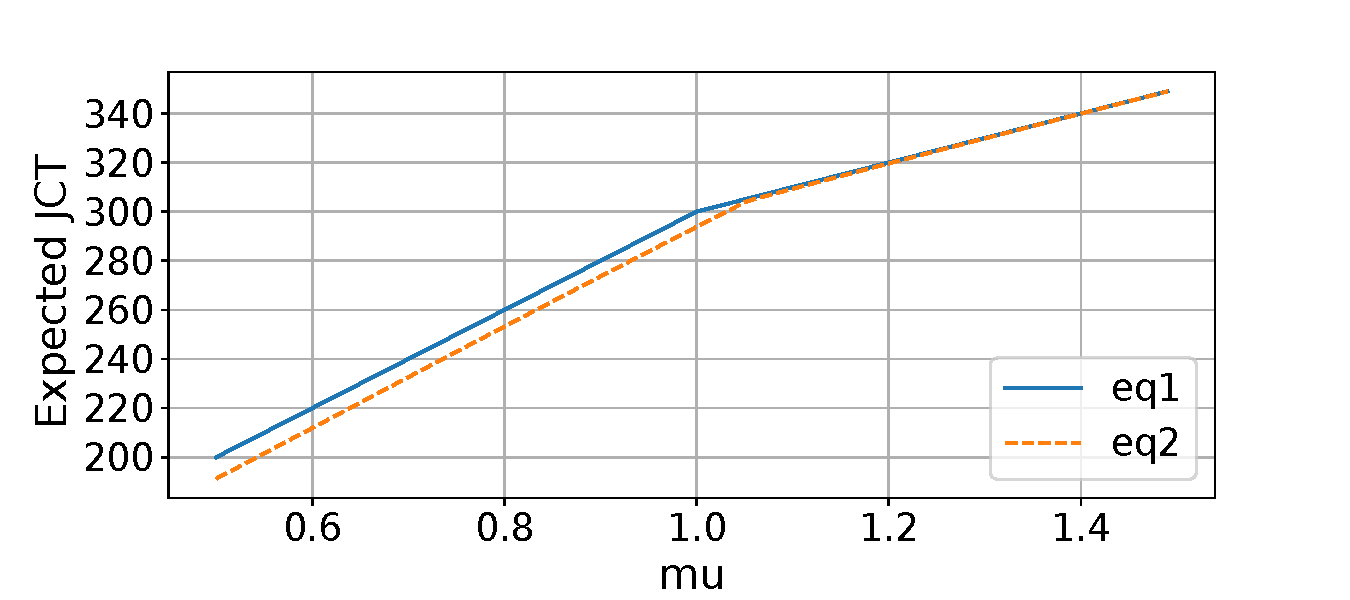
\includegraphics[width=0.9\linewidth]{figures/numerical_analysis/numerical_analysis_0pt5_1pt5_0pt01_sigma0-0pt01_sigma1-1_varying_mu.pdf}
\label{fig:numerical_analysis:variableMu}
}
\subfigure[\vspace{-0.2in} sigma0 = 1 sigma1 = 0.01]
{
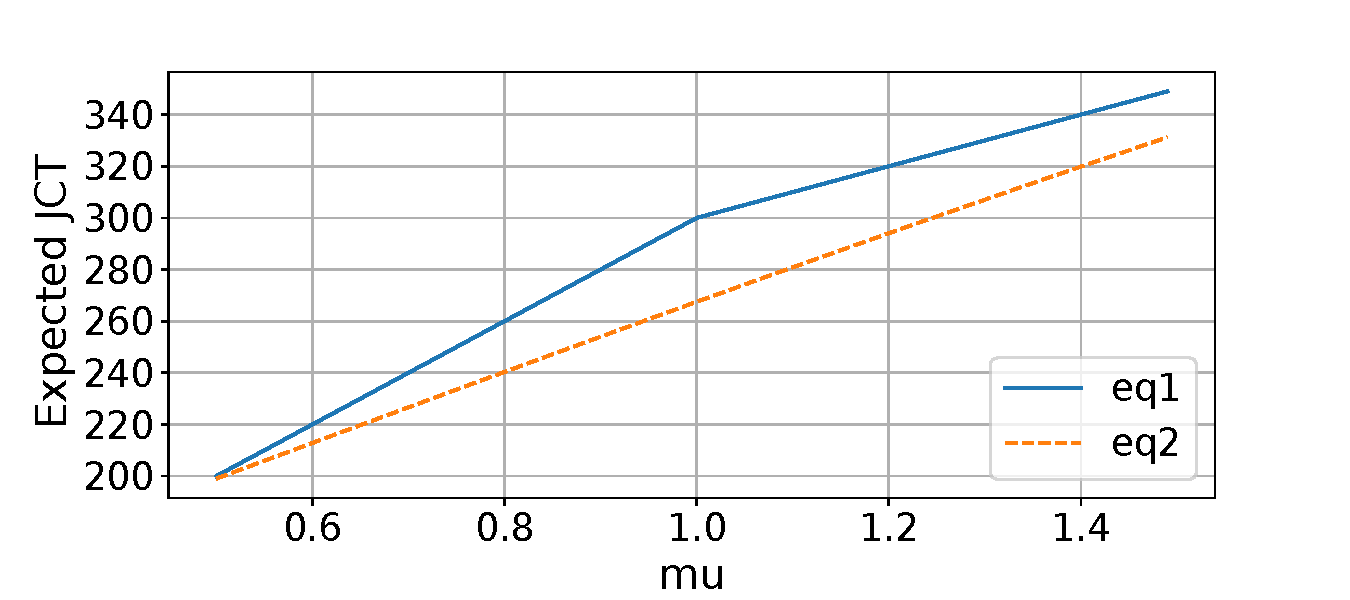
\includegraphics[width=0.9\linewidth]{figures/numerical_analysis/numerical_analysis_0pt5_1pt5_0pt01_sigma0-1_sigma1-0pt01_varying_mu.pdf}
\label{fig:numerical_analysis:variableMu}
}
\caption{Numerical Analysis. Varying $\mu$ from 0.5 to 1.5 with step of 0.01. $m = 5$, $n = 100$.
	\todoaj{Make the y-label as "E[Total JCT]"}
	}
\vspace{-0.1in}
\label{fig:qunatitative_analysis}
\end{figure}
\fi

%\if 0
\begin{table}[tp]
\caption{Summary of trace properties.}
\label{table:traceSummary}
\centering
{\small
\vspace{-0.1in}
\begin{tabular}{|c|c|c|c|c|c|}
\hline
		\textbf{ Trace} & \textbf{Arrival} & \textbf{Resource} & \textbf{Resource}  & \textbf{Indiv. task} \\
			& \textbf{time} & \textbf{requested} & \textbf{usage} & \textbf{duration}\\
	 
\hline
	  \textbf{2Sigma} & Yes & Yes & No & Yes\\
\hline
	  \textbf{Google} & Yes & Yes & Yes & Yes\\
\hline
%\hline
%		\textbf{ Trace} & \textbf{Arrival} & \textbf{Resource} & \textbf{Resource}  & \textbf{Individual} & \textbf{Task success}&{\bf Fraction of}\\
%			& \textbf{time} & \textbf{requested} & \textbf{usage} & \textbf{task duration} & \textbf{status} &{\bf thin jobs}\\
%	 
%\hline
%	  \textbf{2Sigma~\cite{2Sigma:website}} & Yes & Yes & No & Yes & Yes & Relatively low\\
%\hline
%	  \textbf{Google~\cite{googleTraceGithub}} & Yes & Yes & Yes & Yes & Yes & Relatively High\\
%\hline
\end{tabular}
\vspace{-0.1in}
}
\end{table}
%\fi


\subsection{Trace-based Variability Analysis}
\label{sec:accuracy:trace}


Our theoretical analysis in \S\ref{sec:accuracy:quantity} provides 
insights on how the prediction accuracies of the two approaches depend
on the variation of job run times across time and space.
To understand how such variations fare against each other in practice,
we next measure the actual variations
%  in average task runtimes for jobs across history ($\sigmanotsqrd$) and in task
%  runtime across the tasks of the same job (${\sigmaonesqrd}$).
in three production cluster traces, one from 2Sigma~\cite{2Sigma:website} and
two from Google~\cite{googleTraceGithub, googleClusterData2019},
released in 2011 and in 2019, respectively.

\if 0
Several previous work have experimented to
measure variation across history \cite{morpheus, corral, 3Sigma,
jockey:eurosys2012}. We use the technique based on the state-of-the-art
predictor 3Sigma-Predict~\cite{3Sigma}.
\fi

%\paragraph{Traces.} The Google trace is a publicly
%available~\cite{googleTraceGithub}, 29-day long trace
%collected in May 2011 from a Borg~\cite{borg} cell on a cluster of
%approximately 12.5K machines.
%The machines  are highly heterogeneous; 
%they belong to at least
%three different platforms which use different micro-architectures and/or
%memory technologies~\cite{workloadDiversity:atc18}, and
%according to~\cite{googleClusterData2011-2Schema},
%the machines in the same platform can have substantially different clock rates,
%memory speed, and core counts.
%%It has complete information for more than 0.67 million jobs.
%(The trace does not contain actual machine properties. Other details can be
%found in~\cite{googleClusterData2011-2Schema,googleTraceGithub}).
%The second trace is collected from a private datacenter of 2Sigma. The
%cluster uses an internal proprietary job scheduler running on top of a {Mesos
%cluster manager}~\cite{2Sigma:scheduler}. This trace was collected for a period of 7
%months and from  872 machines. The entire trace contains
%approximately 0.4 million jobs.
%    Table \ref{table:traceSummary} summarizes the information available in the traces.
%  that are used in our analysis.
%
%We calculate the variations in task
%runtimes for each job across time and across space as follows.
%Corresponding to each job, we calculate the following 2 values (a)
%Coefficient of variation (CoV) in average task runtimes across time 
%observed at the time of job arrival and, (b) Observed CoV in task runtimes of the job.

\addaj{\paragraph{Traces.} 
 
2Sigma~\cite{2Sigma:website} engineers provided a trace from their cluster on
direct request. The cluster uses an internal proprietary job scheduler running
on top of a {Mesos cluster manager}~\cite{2Sigma:scheduler}. This trace was
collected for a period of 7 months and from  872 machines. The entire trace
contains approximately 0.4 million jobs.  Table \ref{table:traceSummary}
summarizes the information available in the traces that are used in our
analysis.

Also, Google has publicly released two sets of traces, one collected
in May 2011 and another in May 2019~\cite{googleTraceGithub,
  googleClusterData2019}.  The traces have information collected over
a period of 29 (31) days from 1 (8) Borg~\cite{borg} cells for the
2011 (2019) trace and are released in csv (bigquery) format.  The
machines are highly heterogeneous; they belong to at least three
different platforms which use different micro-architectures and/or
memory technologies~\cite{workloadDiversity:atc18}, and according
to~\cite{googleClusterData2011-2Schema}, the machines in the same
platform can have substantially different clock rates, memory speed,
and core counts.  (The trace does not contain actual machine
properties. Other details can be found
in~\cite{googleClusterData2011-2Schema, googleClusterData2019}).  As
mentioned in~\cite{borgTraceAnalysis2019}, Google 2019 trace is very
large and has 2.8 TiB in compressed form and hence Google made it
available only via \textit{bigquery}~\cite{web:googleBigquery}. However, it
is not feasible to perform the analysis in \S\ref{sec:accuracy:trace}
using \textit{bigquery}.
\comment{explain why not???}
Hence we have used only 2011 trace in our
analysis in \S\ref{sec:accuracy:trace}.}


We calculate the variations in task runtimes for each job across time and
across space as follows.

\paragraph{Variation across time.} To measure the variation in average task
runtime for a job across the history, we follow the following prediction
mechanism defined in 3Sigma~\cite{3Sigma}.

As discussed in \S\ref{sec:back:existing}, 3Sigma~\cite{3Sigma} uses
multiple features to identify a job and predicts its runtime using the feature
that gives the least prediction error in the past. We include all six features
used in 3Sigma:
\textit{application name}, \textit{job name}, \textit{user name}
(the owner of the job), \textit{job submission time (day and hour)},
and \textit{resources requested} by the job.
%These are the same set of features as listed in 3Sigma~\cite{3Sigma}.  

% hitory. However, they approximate it as storing entire history will take too much memory.}
For each feature, we define the set of similar jobs as
all the jobs executed in the history window
(defined below) that had the same feature value.
Next, we calculate the average task runtime of each job in the set. Then, we
calculate the {\em Coefficient of Variation} (CoV) of the average task runtimes
across all the jobs in the set. We repeat the above process for all the
features.  We then compare the CoV values thus calculated and pick the minimum
CoV.
% The above procedure is similar in
% principle to the prediction procedure of 3Sigma~\cite{3Sigma}.
Effectively, the above procedure selects the least possible variation
across history.

\paragraph{Varying the history length in prediction across time.}
%\questionaj{The figure \ref{fig:accuracy:trace} is on job count
%window. Will add a day wise figure for \ref{fig:accuracy:trace} too. But there
%we need to have only one fixed window size. We cannot have multiple windows
%there. What do you think we should keep the window size?}
3Sigma used the entire history for prediction.
Intuitively, the length of the history affects the trade-off between
the number of similar jobs and the staleness of the history information.
For this reason, we optimized 3Sigma
by finding and using the history length that gives the least variation.
Specifically, we define the length of history based
on a window size $w$, \ie the number of past consecutive days.
%  In particular, when we calculate the CoVs for a job on day $i+w$,
% the history window starts from day $i$ to day $i+w-1$.
In our analysis below, we vary $w$ among 3, 7, and 14 for the Google trace and 15, 30, 60 and
120 for the 2Sigma trace.
\rm{We start the analysis on the day after the largest window value
  so that we can compare the CoVs for the same jobs when varying the history length.
  }

%   Next, we calculate CoVs in the same way as described
%   above for all the jobs on $i+w+1^{th}$ day using all the jobs in range $i^{th}$
%   to $i+w^{th}$ day as the training data. For each value of $w$ we adjust $i$ such
%   that the set of end days \ie set of $i+w+1^{th}$ days is same for all the three
%   window sizes.
%For one window period we plot one CDF of all the CoVs measured by
%varying the window over it's range. The space curve shows the task CoV.
%$\sqrt{numberOfTasks*0.05}$

\begin{figure*}[tp]
%\vspace{-0.1in}
\centering
\subfigure[Task runtime in the 2Sigma trace]
{
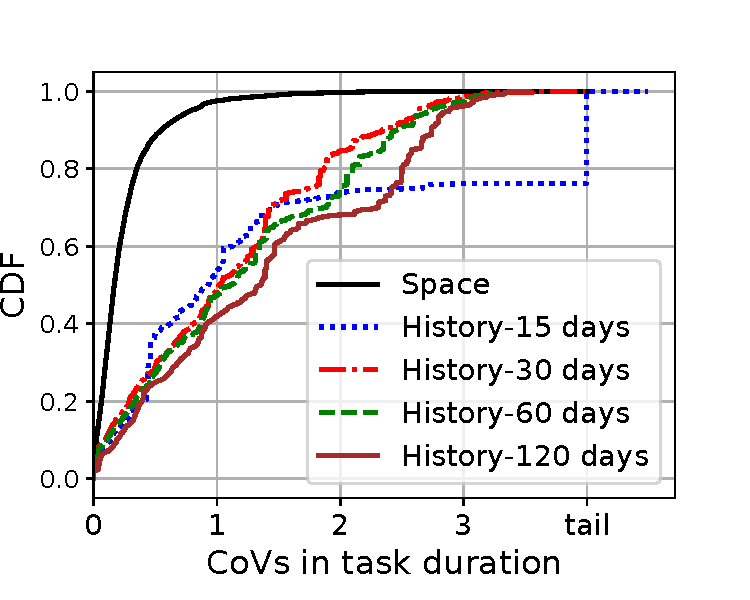
\includegraphics[width=0.25\linewidth]{figures/trace_analysis/slidingWindow_analysis_unified_cdf_of_covs_in_avg_task_runtime_for_user_name_in_2Sigma.pdf}	% done
\label{fig:accuracy:trace_analysis_window:2Sigma:task_dur}
}
\hspace{-15pt}
\subfigure[Task runtime in the Google trace]
{
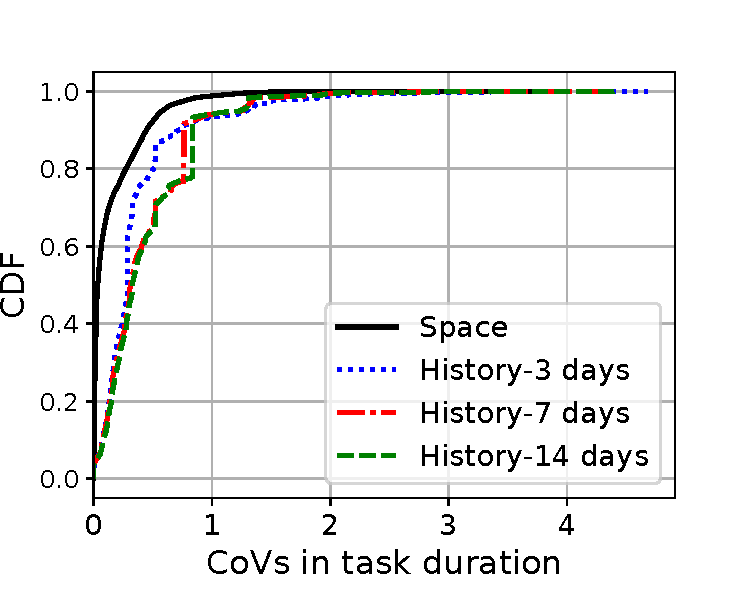
\includegraphics[width=0.25\linewidth]{figures/trace_analysis/slidingWindow_analysis_unified_cdf_of_covs_in_avg_task_dur_for_application_name_in_google11.pdf}	% done
\label{fig:accuracy:trace_analysis_window:google11:task_dur}
}
%\\
\hspace{-15pt}
\vspace{-0.1in}
\subfigure[CPU usage in the Google trace]
{
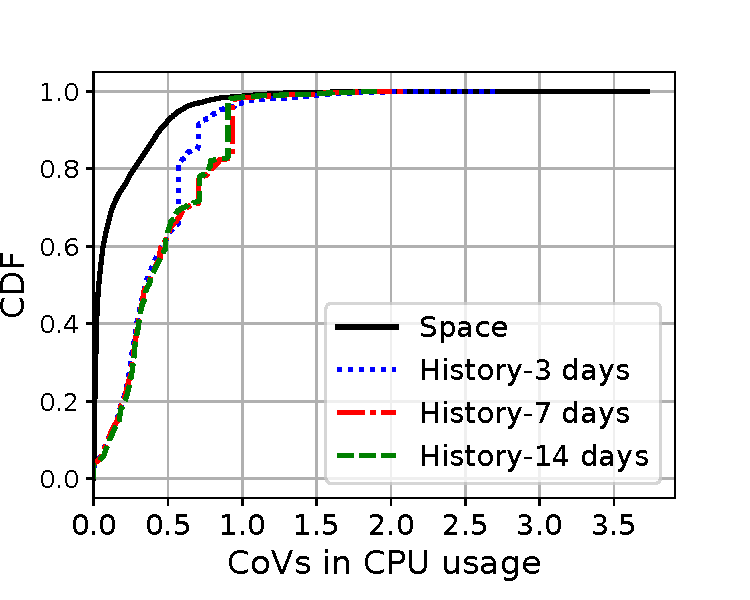
\includegraphics[width=0.25\linewidth]{figures/trace_analysis/slidingWindow_analysis_unified_cdf_of_covs_in_mean_CPU_usage_for_application_name_in_google11.pdf}	% done
\label{fig:accuracy:trace_analysis_window:google11:cpuUsage}
}
\hspace{-15pt}
\subfigure[Disk IO time in the Google trace]
{
%\vspace{-0.2in}
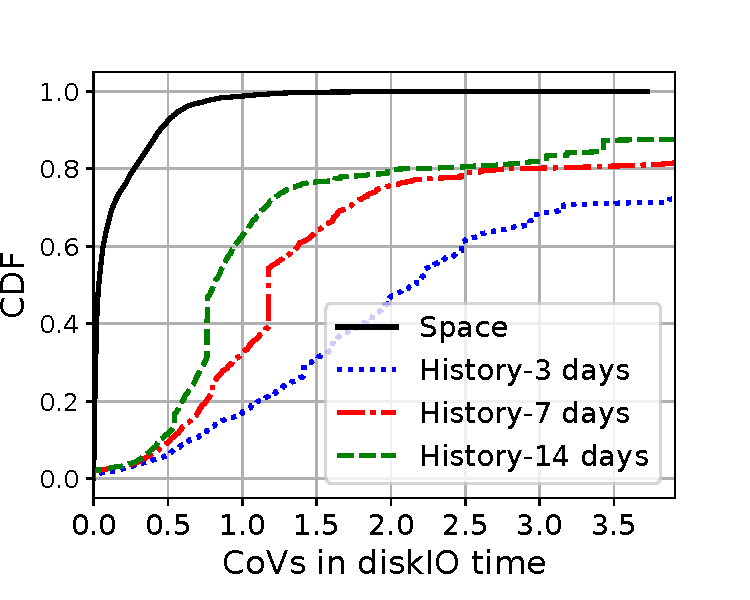
\includegraphics[width=0.25\linewidth]{figures/trace_analysis/slidingWindow_analysis_unified_cdf_of_covs_in_mean_diskIO_time_for_application_name_in_google11.pdf}	% done
\label{fig:accuracy:trace_analysis_window:google11:diskIO}
}
\vspace{-0.1in}
\caption{CDF of CoV of runtime properties 
  across space
  and across time with varying history windows,
          using the 2Sigma and the Google traces.
	  Single-task jobs are excluded from the analysis across space.
%          Figures show coefficient of variation in
%	measured runtime properties of the job. For measuring CoV across time
%	(history) we choose the feature with least variation as described in
%	\S\ref{sec:accuracy:trace}. Also, in case of time we plot the average
%	value of the property of the tasks of a job. For space we plot CoVs
%	across tasks of the job as described in \S\ref{sec:accuracy:trace}. In
%	this analysis we excluded single task jobs. The CDFs are for all the
%	jobs in the window period.Figure
%	\ref{fig:accuracy:trace_analysis_window:google11:cpuUsage} and
%	\ref{fig:accuracy:trace_analysis_window:google11:diskIO} show
          %	variations on CPU usage and disk IO time for the Google trace.
        }
\vspace{-0.1in}
\label{fig:accuracy:trace_analysis_window}
\end{figure*}

\paragraph{Variation across space.} 
To measure the extent of variation across space, we look at the
CoV (CoV $= \frac{\sigma}{\mu}$) in the task
runtimes of a job.  As shown in \S\ref{sec:accuracy:quantity}, the variance in
the task runtime predicted from sampling is $\frac{\sigmaonesqrd}{m}$, where
$\sigmaonesqrd$ is the variance in the runtimes for all the tasks of the job
and $m$ is the number of tasks sampled.  Thus, the observed \textit{CoV} in the
task runtimes of jobs after sampling $m$ tasks becomes
$\frac{\sigmaone/\sqrt{m}}{\mu}$.
%= \frac{cov}{\sqrt{m}}$,
%where $\sigmaone$ is the standard deviation in the runtimes of all the tasks of
%the job, $m$ is the number of tasks sampled (5\% of the total tasks) and $\mu$
%is the average task runtime.
Empirically (\S\ref{sec:sim:numPilots}), we found that sampling 5\% of the
total tasks gives considerably low variation in the predicted tasks runtimes.
Hence, for measuring the extent of variation across space, we plot
$\frac{\sigmaone}{(\sqrt{0.05\times numberOfTasksInJob}\ )\times\mu}$.

\paragraph{Variability comparison.}
{
Fig.~\ref{fig:accuracy:trace_analysis_window:2Sigma:task_dur} and
Fig.~\ref{fig:accuracy:trace_analysis_window:google11:task_dur} show the CDF of CoVs
in task runtimes measured across space and across history for multiple history
window sizes for the complete 2Sigma and Google 2011 traces, respectively.
Table~\ref{table:accuracy:trace_analysis:covs} summarizes the result,
where the CoVs across time correspond to the best history window size,
\ie 30 days for the 2Sigma trace and 3 days for
the Google 2011 trace.
}
Figure~\ref{fig:accuracy:trace_analysis_window:2Sigma:task_dur:scatter}
visualizes the two CoVs for each of 70 randomly selected jobs from the 2Sigma trace in the order of
their arrival, also using the best window size of 30 days.

\rm{For clarity, we first show the result for 70 jobs extracted at
random from the 2Sigma trace, plotted in the order of job arrival in
Figure~\ref{fig:accuracy:trace_analysis_window:2Sigma:task_dur:scatter}.
For each job, we plot the following two values on the y-axis:
%
(1) the CoV in average task runtime for the jobs
in the job's history window, for the feature that gives the least CoV,
using 30-day history window which was found to give the least
variation across history as shown in
Figure\ref{fig:accuracy:trace_analysis_window:2Sigma:task_dur}; and
(2) the CoV in task runtimes of the job.  We see that for both traces, the
variation across history is higher than the variation across tasks for more
than 85\% of the jobs.
}

\begin{figure}[tp]
\vspace{-0.1in}
%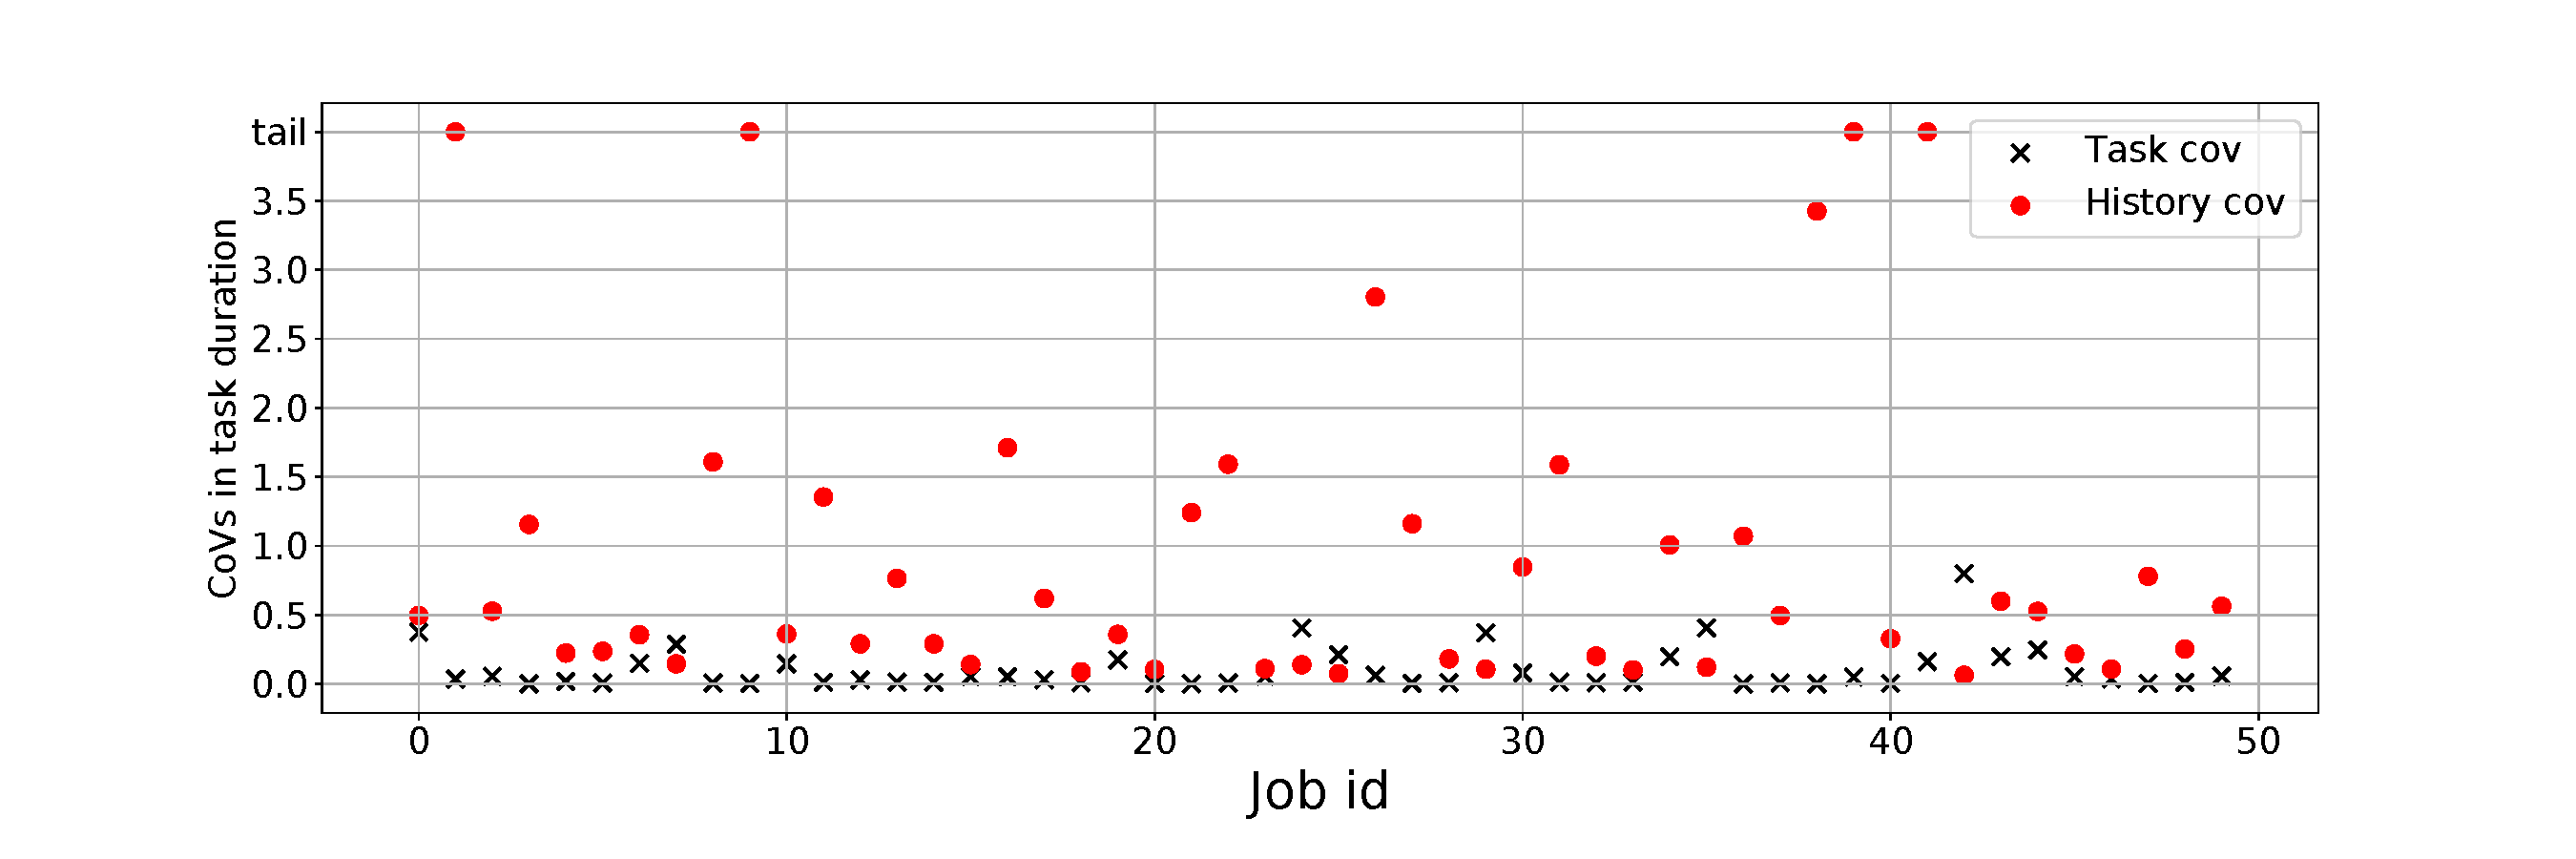
\includegraphics[width=1.0\textwidth]{figures/trace_analysis/slidingWindow_analysis_the_scatter_plot_avg_task_dur_in_google11_initial_history_window_3_days.pdf} %done
%\label{fig:accuracy:trace_analysis_window:google11:task_dur:scatter}
%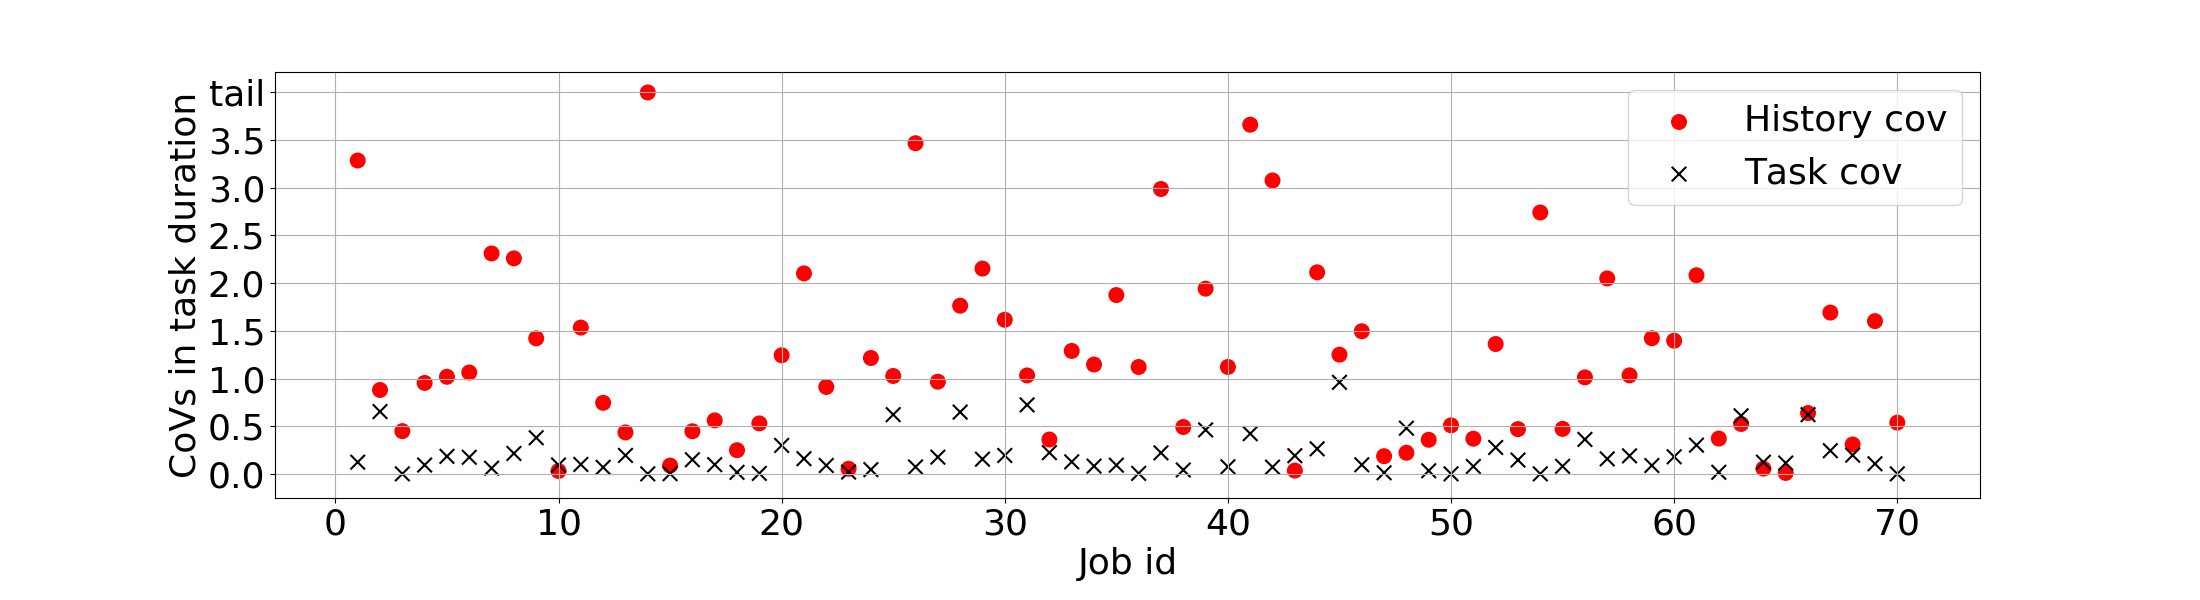
\includegraphics[width=6.5in]{figures/trace_analysis/slidingWindow_analysis_the_scatter_plot_avg_task_runtime_in_2Sigma_initial_history_window_30_days.png} %done
\mbox{\hspace{-0.3in}}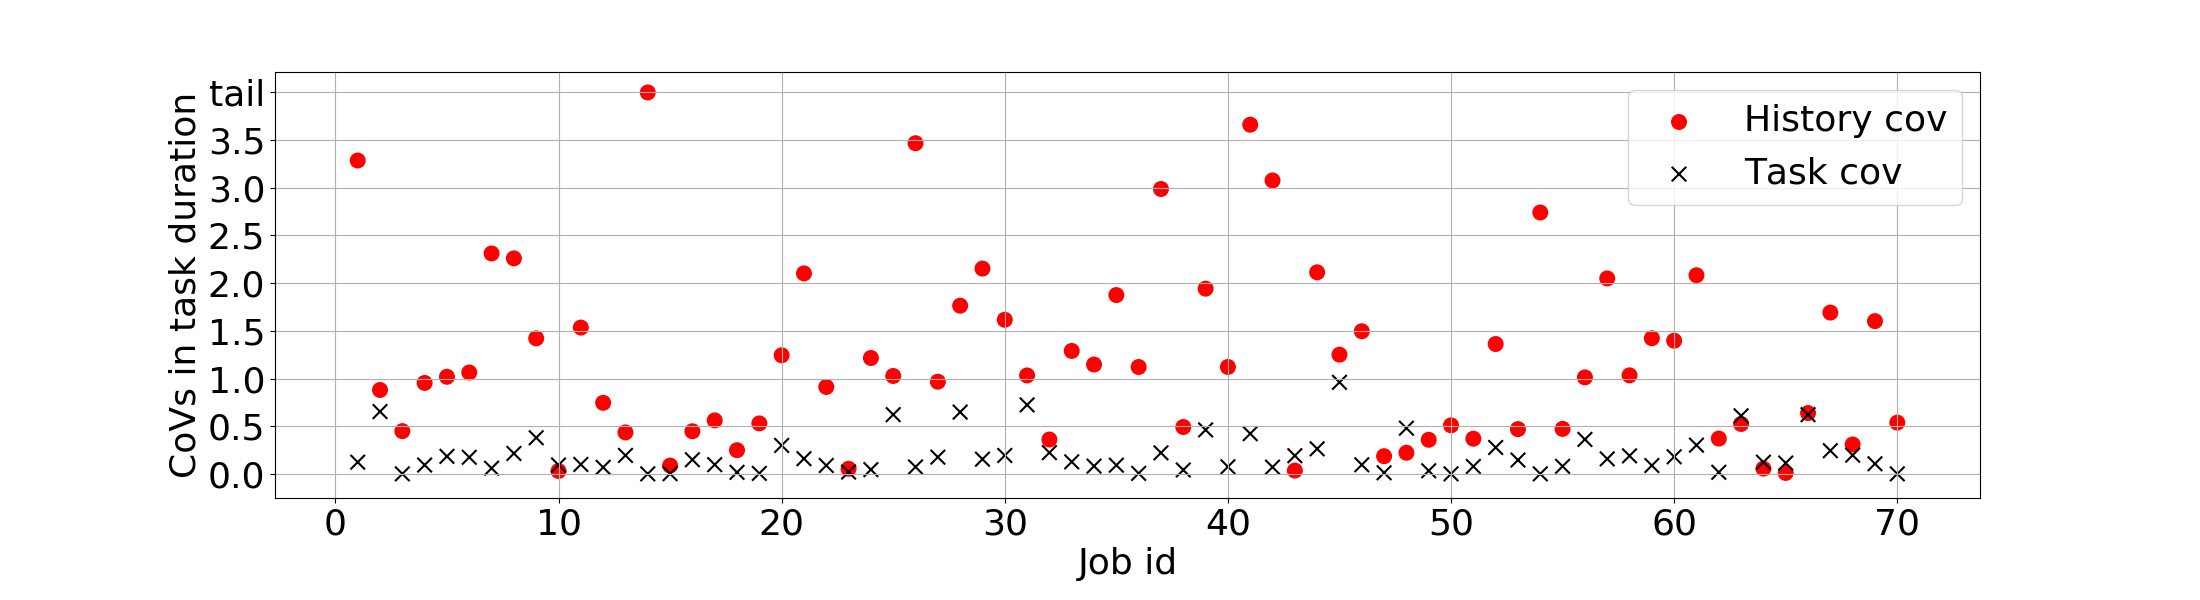
\includegraphics[width=1.2\columnwidth]{figures/trace_analysis/slidingWindow_analysis_the_scatter_plot_avg_task_runtime_in_2Sigma_initial_history_window_30_days.png} %done
%\label{fig:accuracy:trace_analysis_window:2Sigma:task_dur:scatter}
\vspace{-0.25in}
	\caption{CoVs across time and space
	for 70 jobs selected randomly from the 2Sigma trace.
% 	As evident from Figure
%	\ref{fig:accuracy:trace_analysis_window:2Sigma:task_dur} 30-day history
%	window gives lowest CoVs across time so we choose 30 days as history
        %	period to calculate CoVs across time.
        The x-axis represents job ids in the order of their arrival.}
\vspace{-0.1in}
\label{fig:accuracy:trace_analysis_window:2Sigma:task_dur:scatter}
\end{figure}

We see that the P50 (P90) CoV across history is 0.63 (2.99) for the
2Sigma trace and is 0.50 (2.87) for the Google 2011 trace.
%      The high variability across history can be
%      explained as follows. For the Google trace, more than 67\% of the jobs studied
%      were non-recurring, \ie no exact same job was found for them in history, and
%      only 9\% jobs had more than 20\% of all historical jobs as recurring instances.
%      For this analysis, we
%      follow~\cite{corral, morpheus}, and identify two jobs as recurring instances
%      when they have the same jobname and are being executed by the same application.
%      We did
%      not find recurring jobs in the 2Sigma trace. That is what this statement is
%      saying that we were not able to any such information from the 2 Sigma trace.}
%      The lack of a large number of recurring jobs in the histoy window in turn leads
%      to high error in prediction.
In contrast, the P50 (P90) CoV value across the task duration of the
same job is much lower, 0.03 (0.45) for the Google 2011 trace and 0.12 (0.65) for the
2Sigma trace.
%
% {For the 2Sigma (Google) trace, for more than 30\% of the
%   jobs, the CoV across history is at least 10 (35) times higher than the CoV across tasks.
  % for next 20\% it is somewhere between 10-4 (35-15). CoV across history is higher than CoV
% across tasks only for 13\% (16\%) of the jobs.}
%
{For the 2Sigma (Google 2011) trace, the CoV across history is higher than the CoV across
  tasks for 87\% (84\%) of the jobs.
  In particular, for more than 30\% of the jobs,
  the CoV across history is at least 10 (35) times higher than the CoV across tasks.
}
The CoV values across tasks is much lower
because, as
mentioned in the trace schema released by
Google~\cite{googleClusterData2011-2Schema}, the tasks of a job run
exactly the same code with the same flags, settings and priority.
{We confirmed the same is true for the 2Sigma trace
with 2Sigma {engineers}~\cite{personalCommunication:MarkAstley}.  }
% Hence the predictions made by sampling tasks should have a low error.

{Fig.~\ref{fig:accuracy:trace_analysis_window:google11:cpuUsage} and
Fig.~\ref{fig:accuracy:trace_analysis_window:google11:diskIO} further show the
CDF of CoVs for CPU usage and Disk IO time for the Google 2011 trace (such resource
usage is not available in the 2Sigma trace.).
%\addaj{The CoVs here were also measured in the same way as for the task durations.}
%  We use the same
%  methodology for plotting these figures as we did for the task durations.
% We plot in Fig.~\ref{fig:accuracy:trace_analysis_window}
% the variation across space and time for all the jobs in the two traces.
%  For the Google trace, we measure the variation in
%  three runtime properties: Task duration, CPU usage and Disk IO
%  time. In the 2Sigma trace, resource usage is not available and hence
%  we only measured the variation in task duration.
%
The figures show that the variation in the values of these properties when
sampled across space is also considerably lower compared to the variation
observed over time.
}

\begin{table}[tp]
%\vspace{-0.05in}
  \caption{CoV in task runtime across time and across space for the
	the 2Sigmaa and Google 2011 traces.}
\label{table:accuracy:trace_analysis:covs}
\centering
{\small
\vspace{-0.1in}
\begin{tabular}{|c|c|c|c|c|c|}
\hline
                 Trace       & P50 CoV & P90 CoV & P50 CoV & P90 CoV \\
			& (Time)  & (Time)& (Space) & (Space) \\
%\hline
\hline
	2Sigma & 0.63 & 2.99 & 0.12 & 0.65 \\
	 %Trace &  & &      &\\
\hline
	Google & 0.50 & 2.87 & 0.03 & 0.45 \\
	%Trace &    &&&\\
\hline
%\vspace{-0.2in}
\end{tabular}
}
\vspace{-0.1in}
\end{table}

\subsection{Experimental Prediction Error Analysis}
\label{sec:accuracy:experiment}

To validate the analysis from \S\ref{sec:accuracy:quantity} 
that lower task-wise variation than job-wise
variation (\S\ref{sec:accuracy:trace}) will translate into better
prediction accuracy of sampling-based schemes over history-based
schemes, we next implement a sampling-based predictor \slearn and
experimentally compare it against a state-of-the-art history-based
predictor \primarybasepredict~\cite{3Sigma} in estimating the job
runtimes.

%The experimental setup used for this comparison is described below.
\paragraph{Workload characteristics.}
As in 3Sigma~\cite{3Sigma},
we filtered out 3
experimental traces with roughly 1250 jobs each
from the three production cluster traces described in
\S\ref{sec:accuracy:trace}.
We denote the traces extracted
from 2Sigma~\cite{2Sigma:website}, Google 2011 version~\cite{googleTraceGithub}
and Google 2019 version~\cite{googleClusterData2019} 
as 2STrace, GTrace11 and GTrace19, respectively.

\addaj{The 2Sigma trace has many wide jobs and many of them are wider than the number
of nodes (441, each with 24 cores) in the original cluster. Since our
experimental cluster has only 150 single core nodes,
in extracting 2STrace, 
we recalibarated the job widths.  The original 2Sigma trace does not
have exact information on resource usage so we assumed that each task uses 1
core. With this assumption we calculated the effective number of cores per
machine to be 5.49 in order for
the average workload ofthe original trace to remain 1.0 (This
ensures no persistant queue build-up in the cluster). 
Using this effective cluster size, we randomly
dropped some tasks from each job so that the ratio of job width to cluster size remains
the same as ???. We then randomly selected 1250 jobs as the 2STrace.
}

\addaj{To extract GTrace11 and GTrace19, we followed the following process.
  % Based on a suggestion from a Google engineer,
  First, we dropped single
 task jobs from both Google traces for two
  reasons~\cite{personalCommunication:Nan}: (1) these jobs make less
  than 1\% of the total workload, (2) most of these jobs are test jobs
  their performance are not cosidered important.
  %
  Second, since the Google traces do not have
  much wide jobs and the original clusters are very wide, with ~12.5K
  machines, we simply dropped jobs with more than 150 tasks.
  We then randomly selected ~1250 jobs from the Google 2011 trace to create GTrace11.

  To extract GTrace19, we added a few more steps.  First, the Google
  2019 trace had information about the job tier, \eg batch or
  production. Since the SLO for batch tier jobs is to minimize the
  average completion time, we chose batch tier jobs from the 2019
  trace.  Second, the Google 2019 trace has data from eight different
  cells located in 8 different locations. From private
  communication~\cite{personalCommunication:Nan} we learned that {at
    Google, the job properties vary with the social behaviour of
    different locations and it is hard to identify an average cell.
    Given we already had the two two traces from the US, we chooe the
    \textit{clusterG} in the Google 2019 trace which is located in
    Singapore~\cite{googleClusterData2019Schema} as our third trace to
    diversity the loctions of our trace collection.  }

  \if 0
  Another reason to choose the
  \textit{clusterG} from 2019 trace is that, as shown in the trace
  analysis paper~\cite{borgTraceAnalysis2019}, it has highest machine
  utilization and the 2011 trace has machine utilization lower than
  any of the clusters in 2019.
  \fi


\comment{Finally, for each sampled job tacce, we appropriately compressed
    the arrival time of the jobs so that the average cluster load
    remains 1.0, which we assumed is the case in the orignal trace
    as otherwise there would be persistent job queue build-up.
%    is necessary to avoid persistant queueing.
  }

% \addaj{\textbf{Pretraining history based predictors:} Since the experimental traces
% are only 1250 jobs, the history based predictors needs to be pretrained.
Finally, we followed the same process as in~\cite{3Sigma}
To extract pre-training jobs for 3Sigma,
we divided each original traces in chronological
order in two halves, and selected "history" from the first
half and the execution trace defined above from the second half.

\if 0
\paragraph{Workload characteristics.}
{Starting with the two production cluster traces described in
  \S\ref{sec:accuracy:trace}, we filtered out jobs with more than 150
  tasks since our cluster size is 150 nodes.
Following 3Sigma~\cite{3Sigma}, we extracted 1250 jobs from full traces for simulation
and testbed experiments in order to expedite the experiments.
% 
We then extracted two test traces, GTrace and 2STrace, each having
1250 jobs randomly selected from the corresponding filtered
traces. The traces are xx and xx hours long respectively.  For
both of them, we maintain the job arrival time distribution similarly
as in the original traces.  We then extracted corresponding training
data for the history-based predictor \primarybasepredict, which
contains 3,000 jobs each randomly selected from the filtered traces,
using the correspondingly best history windows observed in
\S\ref{sec:accuracy:trace}.
\commentaj{write about trace width compression here.}
\addaj{Write following points: We removed all the single task jobs from the
experimental traces as single task jobs make a very insignificant (less than
0.5\%) portion of the total runtime and resource usage. Samething was confirmed
to us in a personal conversation by a Google engineer that they don't care much
about single task job. Also, in many cases job masters are run as a seperate
single task job.}
\rm{We assume each task in the trace requires one node and zero memory.}
\fi


\paragraph{Prediction mechanisms and experimental setups.}
%\label{subsec:setup}
We simulated a generic job scheduler on a cluster of 150 nodes
that minimizes the average job completion time by using
job runtime estimated by either \lTechnique or \primarybasepredict.
The detailed experimental setup is described in \S\ref{sec:study:design}.
%  Since the goal of this experiment is to
%  compare the prediction accuracy, which is independent of the scheduling mechanism.
%  we skip the scheduling details here.   

In \lTechnique, the number of sampled tasks assigned to a job are
$max(1, 0.05 \cdot S)$, where S is the total number of tasks in the
job. We used 5\% sampling fraction to keep the experimental analysis
the same as the trace analysis
(\S\ref{sec:accuracy:trace}). {We only show the results for wide
  jobs (with \thinLimit or more tasks) as in the complete \slearn design (\S\ref{sec:design:gs}), only
  wide jobs go through the sampling phase.
  }

\questionaj{We need to discuss this. What should we do regarding the sampling
percentage in \S\ref{sec:accuracy:trace} and \S\ref{sec:accuracy:experimental}.
The current value used for figure~\ref{fig:accuracy:trace_analysis_window} and
\ref{fig:accuracy:trace_analysis_window:2Sigma:task_dur:scatter} are. The
values in figure~\ref{fig:sim:estimationAccuracy} are for the adaptive
sampling.}

We implement \primarybasepredict following its description in~\cite{3Sigma}.
After learning the job runtime distribution (\S\ref{sec:accuracy:trace}),
it uses a utility function of the estimated job runtime
associated with every job to derive its estimated runtime from the
distribution, by integrating the utility function
over the entire runtime distribution.
% To ensure correct execution of \primarybasepredict,
We learned the default settings
% in a private communication~\cite{personalCommunication:JunWoo} with
from the authors of 3Sigma~\cite{3Sigma} and kept all the settings
and parameters in our implementation the same 
as in 3Sigma~\cite{3Sigma}.

\begin{figure*}[tp]
\centering
\subfigure[2STrace]
{
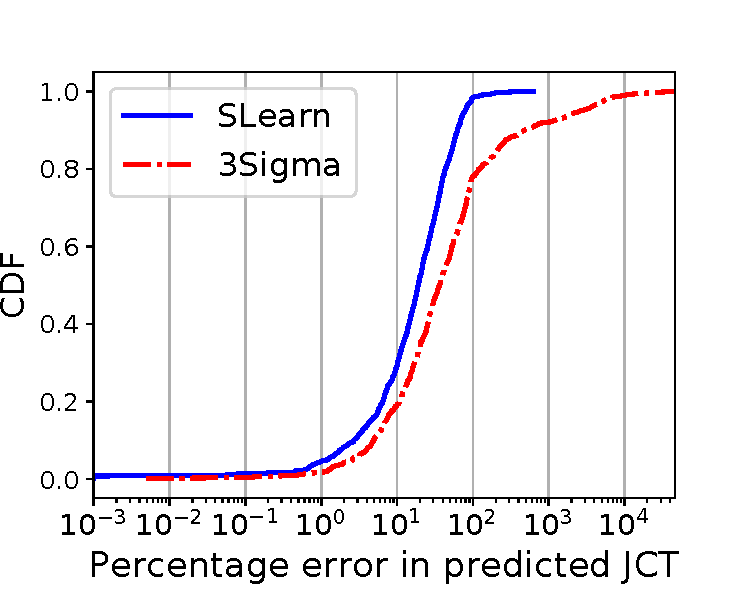
\includegraphics[width=0.33\linewidth]{figures/simulation/prediction_error_new_2STrace.pdf}
%\caption{Job runtime learning accuracy for the 2Sigma trace.}
\label{fig:sim:estimationAccuracy:2STrace}
}
\hspace{-0.25in}
\subfigure[GTrace11]
{
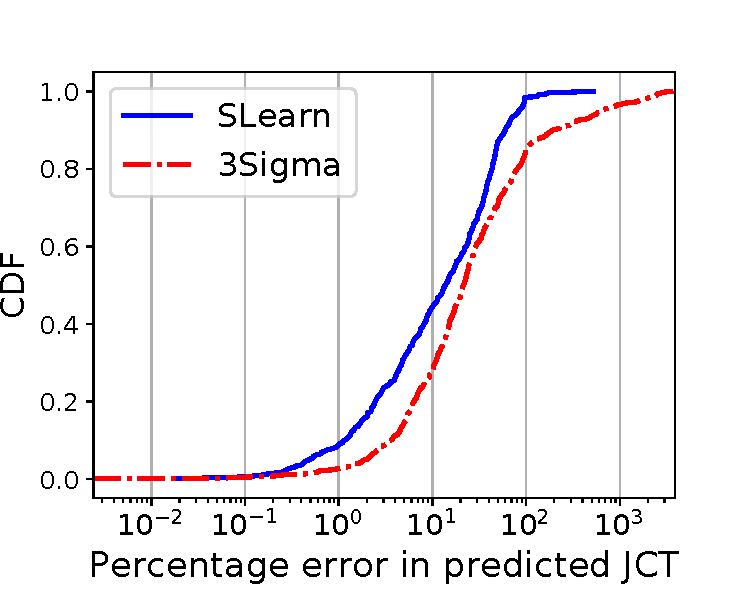
\includegraphics[width=0.33\linewidth]{figures/simulation/prediction_error_new_gTrace.pdf}
\label{fig:sim:estimationAccuracy:GTrace11}
}
\hspace{-0.25in}
\subfigure[GTrace19]
{
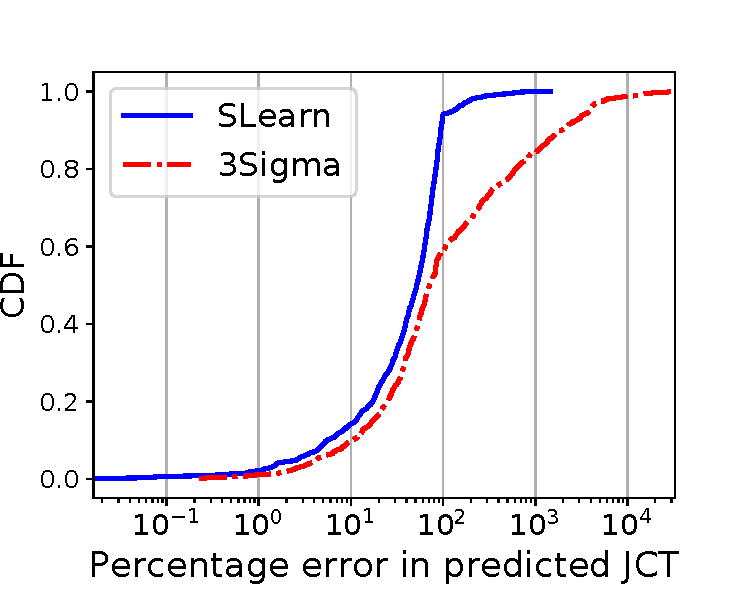
\includegraphics[width=0.33\linewidth]{figures/simulation/prediction_error_new_gTrace2019.pdf}
\label{fig:sim:estimationAccuracy:GTrace19}
}
\vspace{-0.15in}
	\caption{Job runtime prediction accuracy \updated{all - 16th Sep 2020}}
\vspace{-0.15in}
\label{fig:sim:estimationAccuracy}
\end{figure*}

\paragraph{Results.}
Fig.~\ref{fig:sim:estimationAccuracy} shows the percentage error in predicted JCT for 
  the three traces.
% where error = $\frac{abs(predicted\_dur\ -\ actual\_dur)}{actual\_dur}\times100$.
{We see that \slearn has much better prediction accuracy than
  \primarybasepredict.} The P50 error in prediction for 2STrace,
GTrace11, and GTrace19 are 18.98\%, 13.68\%, 51.84\% for \namepredict
but 36.57\%, 21.39\%, 71.56\% for \primarybasepredict, respectively.

\if 0
\commentaj{Cluster G from 2019 has very high error. However, that is not the
case with all the cluster of 2019. I tried with other clusterH with all tier
jobs. That also has a speed up 1.25$\times$ and P50 (P90) error for \slearn is
1.23 (9.39)\% and for \primarybasepredict it is 8.63 (53.60)\%. With clusterB
beb-tier jobs the speedup is 1.9$\times$ and P50 (P90) error for \slearn is
7.65 (58.68)\% and for \primarybasepredict it is 28.72 (144.01)\%. I think we
can use this result somewhere as clusterG 2019 has very high error for both
\slearn and \primarybasepredict.}
\fi

\if 0
{The average prediction error for 2STrace (GTrace) is 27.46 (19.24)\% for \namepredict
but 552.03 (81.35)\%} for \primarybasepredict.
\fi
%  These results
%  show that a sampling-based predictor can predict with better accuracy than the
%  state-of-the-art history-based predictor.

% These results support the conclusion of the quantitative and the trace analysis. 

We observe that the predictor error for 2STrace is higher than for
GTrace11
% which in turn is higher than forGTrace11
for both history-based and sampling-based prediction.  This is because
the 2STrace has higher CoV values for the average task runtimes, both
across the history and across the tasks of the same job
(Table~\ref{table:accuracy:trace_analysis:covs}). This result also
confirms that the prediction accuracy of both schemes are directly
affected by the variance (\S\ref{sec:accuracy:quantity}).
\comment{GTrace19 has the highest prediction errors, though we could
  not analyze its job CoV values due to lack of job information
  (\S\ref{sec:accuracy:trace}).

{To measure the impact of \primarybasepredict's high estimation error in
a job scheduling algorithm, \eg SJF, 
  %  we measured the chances of pairwise order of wide jobs getting
  % swapped from their actual order. \ie
we sorted the jobs in the increasing order of their sizes, and measured how often
the order of each pair of jobs becomes flipped due to incorrect job size
estimation error.  Table~\ref{table:accuracy:trace_analysis:fliprate} shows the
results.  We observe that for the 2STrace, GTrace11, and GTrace19, 23.71\%,
25.83\%, and 39.72\% of job pairs are flipped by \primarybasepredict whereas
only 8.80\%, 13.06\%, and 19.47\% are flipped by \name, respectively.

%  . \ie when runtimesare predicted using \name the chance that the jobs will be sorted in correct
%  order is 94.13\% (91.00\%) for the 2Sigma (Google) trace whereas when
%  \primarybasepredict is used the chances fall down to 78.77\% (76.99\%). If job
%  pairs are to be ordered randomly the chance of correct ordering will be 50\%.
%the chances of flipping are $3.62 \times$ $(2.15 \times)$ higher for the
%\primarybasepredict as compared to the \namepredict
}

\begin{table}[tp]
%\vspace{-0.05in}
  \caption{Chances of correctly ordering pairs of jobs
    for all unique job pairs in each trace.
    %  . We have counted unique pairs. \commentaj{If we show the number of pairs which can flip then it is 2 times for google traces and 3 times for 2 Sigma.} \updated{all - 16th Sep 2020}
  }
\label{table:accuracy:trace_analysis:fliprate}
\centering
{\small
\vspace{-0.1in}
\begin{tabular}{|c|c|c|c|c|c|}
\hline
		 Trace       & \name &  \primarybasepredict & Random\\
			& (Space)  &  (Time) & (No info) \\
%\hline
\hline
	2Sigma & 91.20\%  & 76.29\% & 50.00\% \\
\hline
	Google11 & 86.94\%  & 74.17\% & 50.00\% \\
\hline
	Google19 & 80.53\%  & 60.28\% & 50.00\% \\
\hline
%\vspace{-0.2in}
\end{tabular}
}
\vspace{-0.1in}
\end{table}

In summary, the above quantitative, trace-based and experimental analysis
demonstrate that a sampling-based scheme can predict job runtime
characteristics with considerably higher accuracy than
a state-of-the-art history-based predictor.
